\documentclass[border=4pt,12pt]{standalone}
% House style for redrawn exam diagrams (diagram-v4: 0.4pt lines, filled -latex arrows, fine dashes; stipple and hatching drawn as real dots/lines (no PDF/SVG patterns, so they render in every browser and at any scale); transparent background). Every figure \input's this.
\usepackage{amsmath,amssymb}
\usepackage{txfonts}
\usepackage{pdfrender,xcolor}
% \halo{text}: label on shading. The shading stops just around each letter's outline (a thin knock-out that follows the
% glyphs, like the papers' typesetting), never a box. Owner: "I don't want a box around the text".
\newcommand{\halo}[1]{\leavevmode\rlap{\pdfrender{TextRenderingMode=2,LineWidth=2.2pt,LineJoinStyle=1,StrokeColor=white,FillColor=white}#1}#1}
\usepackage{tikz,pgfplots}
\pgfplotsset{compat=1.18}
\usetikzlibrary{arrows.meta,calc,angles,quotes,patterns,patterns.meta,intersections,positioning,decorations.markings,shapes.geometric}
% Stipple and hatching are drawn as actual dots / lines clipped to the region (path picture), NOT as pattern fills:
% SVG <pattern> fills vanish or blur when browsers scale the image, so the owner could not see the shading.
% Each dot is a 0.72pt square (keeps SVGs small; reads as a dot at print size). Dots sit on one global staggered grid, so neighbouring regions line up.
\makeatletter
\newdimen\ex@x \newdimen\ex@y \newdimen\ex@xa \newdimen\ex@ya \newdimen\ex@xb \newdimen\ex@yb \newcount\ex@row
\def\exam@stipplecolor{black!75}\def\exam@dotr{0.42pt}\def\exam@dotgap{2.5}
\def\ex@rowdots{\ifdim\ex@x<\ex@xb \pgfpathrectangle{\pgfqpoint{\dimexpr\ex@x-0.36pt\relax}{\dimexpr\ex@y-0.36pt\relax}}{\pgfqpoint{0.72pt}{0.72pt}}\advance\ex@x by \exam@dotgap pt\relax\expandafter\ex@rowdots\fi}
\def\exam@stipple{%
  \pgftransformreset% dots are sized in real points even inside scaled pictures
  \pgfpointanchor{path picture bounding box}{south west}\ex@xa=\pgf@x \ex@ya=\pgf@y
  \pgfpointanchor{path picture bounding box}{north east}\ex@xb=\pgf@x \ex@yb=\pgf@y
  \pgfsetfillcolor{\exam@stipplecolor}\pgfmathsetmacro\ex@h{\exam@dotgap/2}%
  \pgfmathtruncatemacro\ex@r{floor(\ex@ya/\ex@h)-1}\ex@row=\ex@r\relax
  \ex@y=\ex@r\dimexpr\ex@h pt\relax
  \loop\ifdim\ex@y<\ex@yb
    \pgfmathtruncatemacro\ex@c{floor(\ex@xa/\exam@dotgap)-1}\ex@x=\ex@c\dimexpr\exam@dotgap pt\relax
    \ifodd\ex@row \advance\ex@x by \ex@h pt\fi
    \ex@rowdots
    \advance\ex@y by \ex@h pt \advance\ex@row by 1
    \ifnum\numexpr\ex@row-(\ex@row/4)*4\relax=0 \pgfusepath{fill}\fi% flush every 4 rows: bounded TeX memory, few clip copies in the SVG
  \repeat\pgfusepath{fill}}
\newdimen\ex@d
\def\exam@hatch#1{% #1 = 1 for /, -1 for \ ; lines 45 degrees, 3pt apart
  \pgftransformreset
  \pgfpointanchor{path picture bounding box}{south west}\ex@xa=\pgf@x \ex@ya=\pgf@y
  \pgfpointanchor{path picture bounding box}{north east}\ex@xb=\pgf@x \ex@yb=\pgf@y
  \ex@d=\dimexpr\ex@yb-\ex@ya\relax \ex@x=\dimexpr\ex@xa-\ex@d\relax
  \loop\ifdim\ex@x<\ex@xb
    \ifnum#1>0 \pgfpathmoveto{\pgfqpoint{\ex@x}{\ex@ya}}\pgfpathlineto{\pgfqpoint{\dimexpr\ex@x+\ex@d\relax}{\ex@yb}}%
    \else \pgfpathmoveto{\pgfqpoint{\ex@x}{\ex@yb}}\pgfpathlineto{\pgfqpoint{\dimexpr\ex@x+\ex@d\relax}{\ex@ya}}\fi
    \advance\ex@x by 4.24pt
  \repeat
  \pgfsetlinewidth{0.4pt}\pgfsetstrokecolor{black}\pgfusepath{stroke}}
\def\examstipple{\exam@stipple}\def\examhatch{\exam@hatch}\def\examsetstipplecolor#1{\def\exam@stipplecolor{#1}}\def\examsetdotgap#1{\def\exam@dotgap{#1}}
\makeatother
% (legacy pattern kept for old files)
% staggered stipple like the NESA papers' dotted shading
\pgfdeclarepatternformonly{exam stipple}{\pgfpointorigin}{\pgfqpoint{2.2pt}{2.2pt}}{\pgfqpoint{2.2pt}{2.2pt}}{%
  \pgfpathcircle{\pgfqpoint{0.55pt}{0.55pt}}{0.42pt}\pgfpathcircle{\pgfqpoint{1.65pt}{1.65pt}}{0.42pt}\pgfusepath{fill}}
\tikzset{
  every picture/.style={line width=0.6pt, >={Latex[length=2mm,width=1.3mm]}},
  curve/.style={line width=0.6pt},
  open arrow/.style={-{Latex[length=2mm,width=1.3mm]}},  % owner: filled -latex heads everywhere, no open chevrons
  aux/.style={dash pattern=on 2pt off 1.5pt, line width=0.6pt},
  shade/.code={\def\exA{#1}\def\exB{none}\ifx\exA\exB\else\pgfkeysalso{fill=black!18}\fi},
  shade/.default=on,
  shade dots/.style={fill=none, path picture={\examstipple}},
  stipple color/.code={\examsetstipplecolor{#1}},
  stipple gap/.code={\examsetdotgap{#1}},
  shade dense dots/.style={fill=none, stipple gap=1.6, path picture={\examstipple}},
  shade hatch/.style={fill=none, path picture={\examhatch{1}}},
  shade hatch reverse/.style={fill=none, path picture={\examhatch{-1}}},
  shade solid/.style={fill=black},
  pt/.style={circle, fill, inner sep=1.1pt},
  open pt/.style={circle, draw, fill=white, inner sep=1.1pt},
}
\pgfplotsset{
  exam axes/.style={axis lines=middle, axis line style={->}, xlabel={$x$}, ylabel={$y$},
    xlabel style={anchor=west}, ylabel style={anchor=south}, tick label style={font=\small},
    every axis plot/.append style={line width=0.6pt, black}, samples=200, clip=false,
    enlargelimits=false, axis on top},
}

\begin{document}
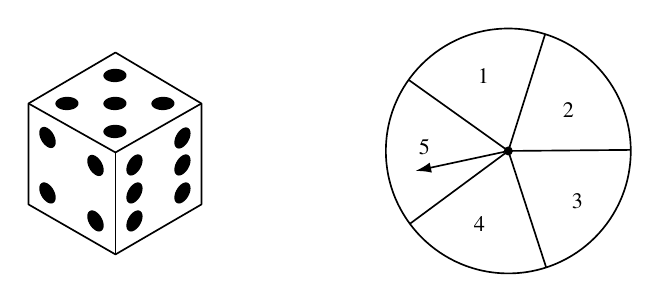
\begin{tikzpicture}[x=0.0127cm,y=-0.0127cm]
\draw[line join=round] (146,48)--(232,99)--(232,200)--(146,250)--(59,200)--(59,99)--cycle; \draw (59,99)--(146,148)--(232,99); \draw (146,148)--(146,250);
\fill plot[smooth cycle] coordinates {(153.7,66.2) (155.3,67.4) (156.4,68.7) (157.0,70.1) (157.0,71.6) (156.4,73.1) (155.3,74.4) (153.7,75.6) (151.7,76.6) (149.3,77.2) (146.8,77.6) (144.2,77.6) (141.7,77.3) (139.3,76.7) (137.3,75.8) (135.7,74.6) (134.6,73.3) (134.0,71.9) (134.0,70.4) (134.6,68.9) (135.7,67.6) (137.3,66.4) (139.3,65.4) (141.7,64.8) (144.2,64.4) (146.8,64.4) (149.3,64.7) (151.7,65.3)};
\fill plot[smooth cycle] coordinates {(105.7,94.2) (107.3,95.4) (108.4,96.7) (109.0,98.1) (109.0,99.6) (108.4,101.1) (107.3,102.4) (105.7,103.6) (103.7,104.6) (101.3,105.2) (98.8,105.6) (96.2,105.6) (93.7,105.3) (91.3,104.7) (89.3,103.8) (87.7,102.6) (86.6,101.3) (86.0,99.9) (86.0,98.4) (86.6,96.9) (87.7,95.6) (89.3,94.4) (91.3,93.4) (93.7,92.8) (96.2,92.4) (98.8,92.4) (101.3,92.7) (103.7,93.3)};
\fill plot[smooth cycle] coordinates {(153.7,94.2) (155.3,95.4) (156.4,96.7) (157.0,98.1) (157.0,99.6) (156.4,101.1) (155.3,102.4) (153.7,103.6) (151.7,104.6) (149.3,105.2) (146.8,105.6) (144.2,105.6) (141.7,105.3) (139.3,104.7) (137.3,103.8) (135.7,102.6) (134.6,101.3) (134.0,99.9) (134.0,98.4) (134.6,96.9) (135.7,95.6) (137.3,94.4) (139.3,93.4) (141.7,92.8) (144.2,92.4) (146.8,92.4) (149.3,92.7) (151.7,93.3)};
\fill plot[smooth cycle] coordinates {(201.7,94.2) (203.3,95.4) (204.4,96.7) (205.0,98.1) (205.0,99.6) (204.4,101.1) (203.3,102.4) (201.7,103.6) (199.7,104.6) (197.3,105.2) (194.8,105.6) (192.2,105.6) (189.7,105.3) (187.3,104.7) (185.3,103.8) (183.7,102.6) (182.6,101.3) (182.0,99.9) (182.0,98.4) (182.6,96.9) (183.7,95.6) (185.3,94.4) (187.3,93.4) (189.7,92.8) (192.2,92.4) (194.8,92.4) (197.3,92.7) (199.7,93.3)};
\fill plot[smooth cycle] coordinates {(153.7,122.2) (155.3,123.4) (156.4,124.7) (157.0,126.1) (157.0,127.6) (156.4,129.1) (155.3,130.4) (153.7,131.6) (151.7,132.6) (149.3,133.2) (146.8,133.6) (144.2,133.6) (141.7,133.3) (139.3,132.7) (137.3,131.8) (135.7,130.6) (134.6,129.3) (134.0,127.9) (134.0,126.4) (134.6,124.9) (135.7,123.6) (137.3,122.4) (139.3,121.4) (141.7,120.8) (144.2,120.4) (146.8,120.4) (149.3,120.7) (151.7,121.3)};
\fill plot[smooth cycle] coordinates {(86.2,137.6) (86.0,139.6) (85.4,141.3) (84.4,142.5) (83.1,143.3) (81.5,143.6) (79.8,143.3) (78.0,142.5) (76.2,141.2) (74.5,139.6) (72.9,137.6) (71.6,135.3) (70.6,133.0) (70.0,130.6) (69.8,128.4) (70.0,126.4) (70.6,124.7) (71.6,123.5) (72.9,122.7) (74.5,122.4) (76.2,122.7) (78.0,123.5) (79.8,124.8) (81.5,126.4) (83.1,128.4) (84.4,130.7) (85.4,133.0) (86.0,135.4)};
\fill plot[smooth cycle] coordinates {(134.2,165.6) (134.0,167.6) (133.4,169.3) (132.4,170.5) (131.1,171.3) (129.5,171.6) (127.8,171.3) (126.0,170.5) (124.2,169.2) (122.5,167.6) (120.9,165.6) (119.6,163.3) (118.6,161.0) (118.0,158.6) (117.8,156.4) (118.0,154.4) (118.6,152.7) (119.6,151.5) (120.9,150.7) (122.5,150.4) (124.2,150.7) (126.0,151.5) (127.8,152.8) (129.5,154.4) (131.1,156.4) (132.4,158.7) (133.4,161.0) (134.0,163.4)};
\fill plot[smooth cycle] coordinates {(86.2,193.1) (86.0,195.1) (85.4,196.8) (84.4,198.0) (83.1,198.8) (81.5,199.1) (79.8,198.8) (78.0,198.0) (76.2,196.7) (74.5,195.1) (72.9,193.1) (71.6,190.8) (70.6,188.5) (70.0,186.1) (69.8,183.9) (70.0,181.9) (70.6,180.2) (71.6,179.0) (72.9,178.2) (74.5,177.9) (76.2,178.2) (78.0,179.0) (79.8,180.3) (81.5,181.9) (83.1,183.9) (84.4,186.2) (85.4,188.5) (86.0,190.9)};
\fill plot[smooth cycle] coordinates {(134.2,221.1) (134.0,223.1) (133.4,224.8) (132.4,226.0) (131.1,226.8) (129.5,227.1) (127.8,226.8) (126.0,226.0) (124.2,224.7) (122.5,223.1) (120.9,221.1) (119.6,218.8) (118.6,216.5) (118.0,214.1) (117.8,211.9) (118.0,209.9) (118.6,208.2) (119.6,207.0) (120.9,206.2) (122.5,205.9) (124.2,206.2) (126.0,207.0) (127.8,208.3) (129.5,209.9) (131.1,211.9) (132.4,214.2) (133.4,216.5) (134.0,218.9)};
\fill plot[smooth cycle] coordinates {(221.1,128.9) (220.9,131.1) (220.3,133.5) (219.3,135.8) (218.0,138.1) (216.5,140.1) (214.8,141.7) (213.0,143.0) (211.2,143.8) (209.5,144.1) (208.0,143.8) (206.7,143.0) (205.7,141.8) (205.1,140.1) (204.9,138.1) (205.1,135.9) (205.7,133.5) (206.7,131.2) (208.0,128.9) (209.5,126.9) (211.2,125.3) (213.0,124.0) (214.8,123.2) (216.5,122.9) (218.0,123.2) (219.3,124.0) (220.3,125.2) (220.9,126.9)};
\fill plot[smooth cycle] coordinates {(221.1,155.9) (220.9,158.1) (220.3,160.5) (219.3,162.8) (218.0,165.1) (216.5,167.1) (214.8,168.7) (213.0,170.0) (211.2,170.8) (209.5,171.1) (208.0,170.8) (206.7,170.0) (205.7,168.8) (205.1,167.1) (204.9,165.1) (205.1,162.9) (205.7,160.5) (206.7,158.2) (208.0,155.9) (209.5,153.9) (211.2,152.3) (213.0,151.0) (214.8,150.2) (216.5,149.9) (218.0,150.2) (219.3,151.0) (220.3,152.2) (220.9,153.9)};
\fill plot[smooth cycle] coordinates {(221.1,183.9) (220.9,186.1) (220.3,188.5) (219.3,190.8) (218.0,193.1) (216.5,195.1) (214.8,196.7) (213.0,198.0) (211.2,198.8) (209.5,199.1) (208.0,198.8) (206.7,198.0) (205.7,196.8) (205.1,195.1) (204.9,193.1) (205.1,190.9) (205.7,188.5) (206.7,186.2) (208.0,183.9) (209.5,181.9) (211.2,180.3) (213.0,179.0) (214.8,178.2) (216.5,177.9) (218.0,178.2) (219.3,179.0) (220.3,180.2) (220.9,181.9)};
\fill plot[smooth cycle] coordinates {(173.1,155.9) (172.9,158.1) (172.3,160.5) (171.3,162.8) (170.0,165.1) (168.5,167.1) (166.8,168.7) (165.0,170.0) (163.2,170.8) (161.5,171.1) (160.0,170.8) (158.7,170.0) (157.7,168.8) (157.1,167.1) (156.9,165.1) (157.1,162.9) (157.7,160.5) (158.7,158.2) (160.0,155.9) (161.5,153.9) (163.2,152.3) (165.0,151.0) (166.8,150.2) (168.5,149.9) (170.0,150.2) (171.3,151.0) (172.3,152.2) (172.9,153.9)};
\fill plot[smooth cycle] coordinates {(173.1,183.9) (172.9,186.1) (172.3,188.5) (171.3,190.8) (170.0,193.1) (168.5,195.1) (166.8,196.7) (165.0,198.0) (163.2,198.8) (161.5,199.1) (160.0,198.8) (158.7,198.0) (157.7,196.8) (157.1,195.1) (156.9,193.1) (157.1,190.9) (157.7,188.5) (158.7,186.2) (160.0,183.9) (161.5,181.9) (163.2,180.3) (165.0,179.0) (166.8,178.2) (168.5,177.9) (170.0,178.2) (171.3,179.0) (172.3,180.2) (172.9,181.9)};
\fill plot[smooth cycle] coordinates {(173.1,211.9) (172.9,214.1) (172.3,216.5) (171.3,218.8) (170.0,221.1) (168.5,223.1) (166.8,224.7) (165.0,226.0) (163.2,226.8) (161.5,227.1) (160.0,226.8) (158.7,226.0) (157.7,224.8) (157.1,223.1) (156.9,221.1) (157.1,218.9) (157.7,216.5) (158.7,214.2) (160.0,211.9) (161.5,209.9) (163.2,208.3) (165.0,207.0) (166.8,206.2) (168.5,205.9) (170.0,206.2) (171.3,207.0) (172.3,208.2) (172.9,209.9)};
\draw (539,146.5) circle[radius=122.5];
\draw (539,146.5) -- ++(-0.5:122.5);
\draw (539,146.5) -- ++(-72.5:122.5);
\draw (539,146.5) -- ++(-144.5:122.5);
\draw (539,146.5) -- ++(-216.5:122.5);
\draw (539,146.5) -- ++(-288:122.5);
\draw[->] (539,146.5) -- (446,166.5);
\fill (539,146.5) circle[radius=4.5];
\node[font=\footnotesize] at (514,72) {1};
\node[font=\footnotesize] at (599,106) {2};
\node[font=\footnotesize] at (608,197) {3};
\node[font=\footnotesize] at (510,220) {4};
\node[font=\footnotesize] at (455,143) {5};
\end{tikzpicture}
\end{document}
